% Autogenerated translation of index.md by Texpad
% To stop this file being overwritten during the typeset process, please move or remove this header

\documentclass[a4paper, 12pt]{book}
\usepackage{graphicx}
\usepackage[utf8]{inputenc}
\usepackage[a4paper]{geometry}
\usepackage{hyperref}
\pagestyle{plain}
\begin{document}

\hrule
layout: default

\section*{title: Physics 426 Fluid Mechanics}

\section*{Physics 426 Fluid Mechanics}

Spring 2016

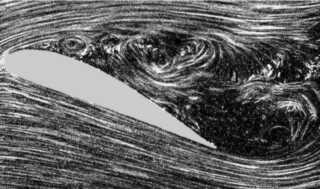
\includegraphics{./figs/Flow_separation.jpg}

\begin{itemize}
\item Instructor: \href{http://web.uvic.ca/~jklymak}{Jody Klymak}
\item Office: \href{http://www.uvic.ca/buildings/sci.html}{Bob Wright Centre} A313
\item Tel: (250)-472-5969; Email: \href{mailto:jklymak@uvic.ca}{jklymak@uvic.ca}
\item Office Hours: Tue 14:30-15:30 or by appointment
\item Meeting time:  TWF 11:30-12:20
\item Location:  \href{http://www.uvic.ca/home/about/campus-info/maps/maps/ell.php}{Ell 161}
\end{itemize}

\section*{Course Objectives}

\begin{itemize}
\item Learn the fundamental properties of fluids.
\item Apply conservation laws to theoretical and practical problems
\item Gain experience with laboratory methods
\item Gain experience in written and spoken presentation
\end{itemize}

\section*{Schedule}

\begin{verbatim}
<iframe width="600px" height="400px" src="https://docs.google.com/spreadsheets/d/e/2PACX-1vQZ2Tmi8zGX8pCgSrf4jDAN--9LXhwSyRjWPwHj0FItENDdJViT87eE4DAOwWnYEGovikh0_GRfHFvP/pubhtml?gid=0&amp;single=true&amp;widget=true&amp;headers=false"></iframe>

\end{verbatim}

\section*{\href{./Texts/}{Texts}}

Largely \href{http://app.knovel.com/web/toc.v/cid:kpFME00004/viewerType:toc/root_slug:fluid-mechanics-4th}{Kundu and Cohen}, 4th edition, but also see \href{./Texts/}{Texts}.  

\section*{Course grading}

5\% Readings/Class Participation; 30\% \href{#Assignments}{Assignments}; 35\% \href{./LabProject/}{Laboratory Project}; 30\% Final Exam

Late work penalized as 10\% per day, max 5 days.  Academic concessions will be granted
with appropriate documentation as per \href{http://www.uvic.ca/registrar/students/policies/appeals/rac-request.php}{UVic's regulations}.

\section*{\href{./LabProject/}{Laboratory Project}}

\section*{Assignments}

\begin{itemize}
\item \href{./Assignments/Assignment1.pdf}{Assignment 1: Due 3 Feb, 11:30 AM}    \href{./Assignments/Assignment1Key.pdf}{Key}
\item \href{./Assignments/Assignment2.pdf}{Assignment 2: Due 22 Feb, 11:30 AM}   \href{./Assignments/Assignment2Key.pdf}{Key}
\item \href{./Assignments/Assignment3.pdf}{Assignment 3: Due 15 Mar, 11:30 AM}    \href{./Assignments/Assignment3Key.pdf}{Key}
\item \href{./Assignments/Assignment4.pdf}{Assignment 4: Due 4 Apr, 11:30 AM}
\end{itemize}

\section*{Take Home final:}

\begin{itemize}
\item \href{./Assignments/TakeHome17.pdf}{Take Home Final: Due 11 Apr, 10:00 AM}
\end{itemize}

\section*{Course Evaluation Survey}

These are filled out online at \href{http://ces.uvic.ca}{ces.uvic.ca}.  There should be a link to this course on your dashboard.

\section*{Mailing list}

Please feel free to contact me through the mailing lists:

\href{mailto:201701-phys426-22537@lists.uvic.ca}{201701-phys426-22537@lists.uvic.ca}

To manage your list, have a look at the appropriate page:

\href{https://lists.uvic.ca/mailman/listinfo/201701-phys426-22537}{https://lists.uvic.ca/mailman/listinfo/201701-phys426-22537}

Questions that will benefit all your classmates are very welcome on
the list.

\end{document}
